\documentclass{beamer}
\usepackage{hyperref} % URLs
\title[Critical Thinking]{Science, truth, and honesty }
%\subtitle[short]{full}
\author{Andy J. Wills}

\date{\today}

\begin{document}
%%%%% All images from wikimedia commons.
\frame{\titlepage}

\begin{frame}{Topics}
	\begin{itemize}
		\item What is truth? 
		\item What is science?  
	\end{itemize}
	\centerline{
	
\includegraphics[width=.3\textwidth]{truth.jpg}
	
\includegraphics[width=.3\textwidth]{science.png}
	}
\end{frame}

\begin{frame}{Truth as a property of claims}
	\begin{itemize}
		\item Statements about truth
		\begin{itemize}
			\item ``Andy is in Plymouth'' $\to$ TRUE 
			\item ``Andy is on the Moon'' $\to$ FALSE 
		\end{itemize}
		\item Statements about the limits of our knowledge
		\begin{itemize}
			\item ``Andy was born in the month of June'' $\to P(true) = 1/12$ 
			\item ``Andy has \pounds 3.57 in his pocket'' $\to$ UNKNOWN
		\end{itemize}  
	\end{itemize}
\end{frame}

\begin{frame}{Subjective and objective claims}
	\begin{itemize}
		\item \textbf{Subjective claims} are those whose truth differs for different people.
		\item ``My favourite colour is blue''
		\item \textbf{Objective claims} are those whose truth value is not affected by who says it.
		\item ``Charlotte Smith's favourite colour is blue''
		\item The term \emph{subjective} is widely misused.
		\item ``I think chocolate tastes better than cabbage'' is subjective.
		\item ``Chocolate tastes better than cabbage'' is objective, and is amenable to scientific test.
	\end{itemize}
\end{frame}

\begin{frame}{Vague claims are subjective}
\begin{itemize}
\item ``Smoking is wrong'' - Subjective.
\item ``Smoking increases life expectancy'' - Objective.
\item Note: Claims do not need to be correct to be objective.
\end{itemize}
\end{frame}


\begin{frame}{What is truth?}
	\begin{itemize}
		\item ``What does it mean to say that an objective claim is true?''
		\item \textbf{Relativism}
		\begin{itemize}
			\item There are no objective claims.
			\item All claims are subjective.
			\item The truth value of of all claims depends on who is speaking them.
			\item \textbf{The truth is relative to different cultures or societies}.
		\end{itemize}
		\item Problems with relativism
		\begin{itemize}
			\item Any definition of relativism is self-defeating
			\begin{itemize}
				\item ``All truth is relative''
				\item This claim is, in itself, universal and so proves that not all truth is relative.
				\item Similarly, ``no one can say what is right or wrong''
			\end{itemize}
			\item Relativism seems to preclude the possibility of being wrong. 	
		\end{itemize}
		\item Weak relativism
		\begin{itemize}
			\item ``some truth is relative''
			\item Uncontentious - see subjective claims
		\end{itemize}
			\item What does it mean to say that an objective claim is true?
	\end{itemize}
\end{frame}

\begin{frame}{Truth, correspondence, and coherence}
	\begin{itemize}
		\item Correspondence Theory 
		\begin{itemize}
			\item Truth is determined by the correspondence between what is claimed and what is observed.
			\item A murder suspect claims to have been at home between 10pm and midnight...
			\item ...but he was seen by a reliable witness some miles from his house at that time.
			\item The suspect's objective claim is judged to be false because it does not correspond to observations.
		\end{itemize}
	\end{itemize}
	\centerline{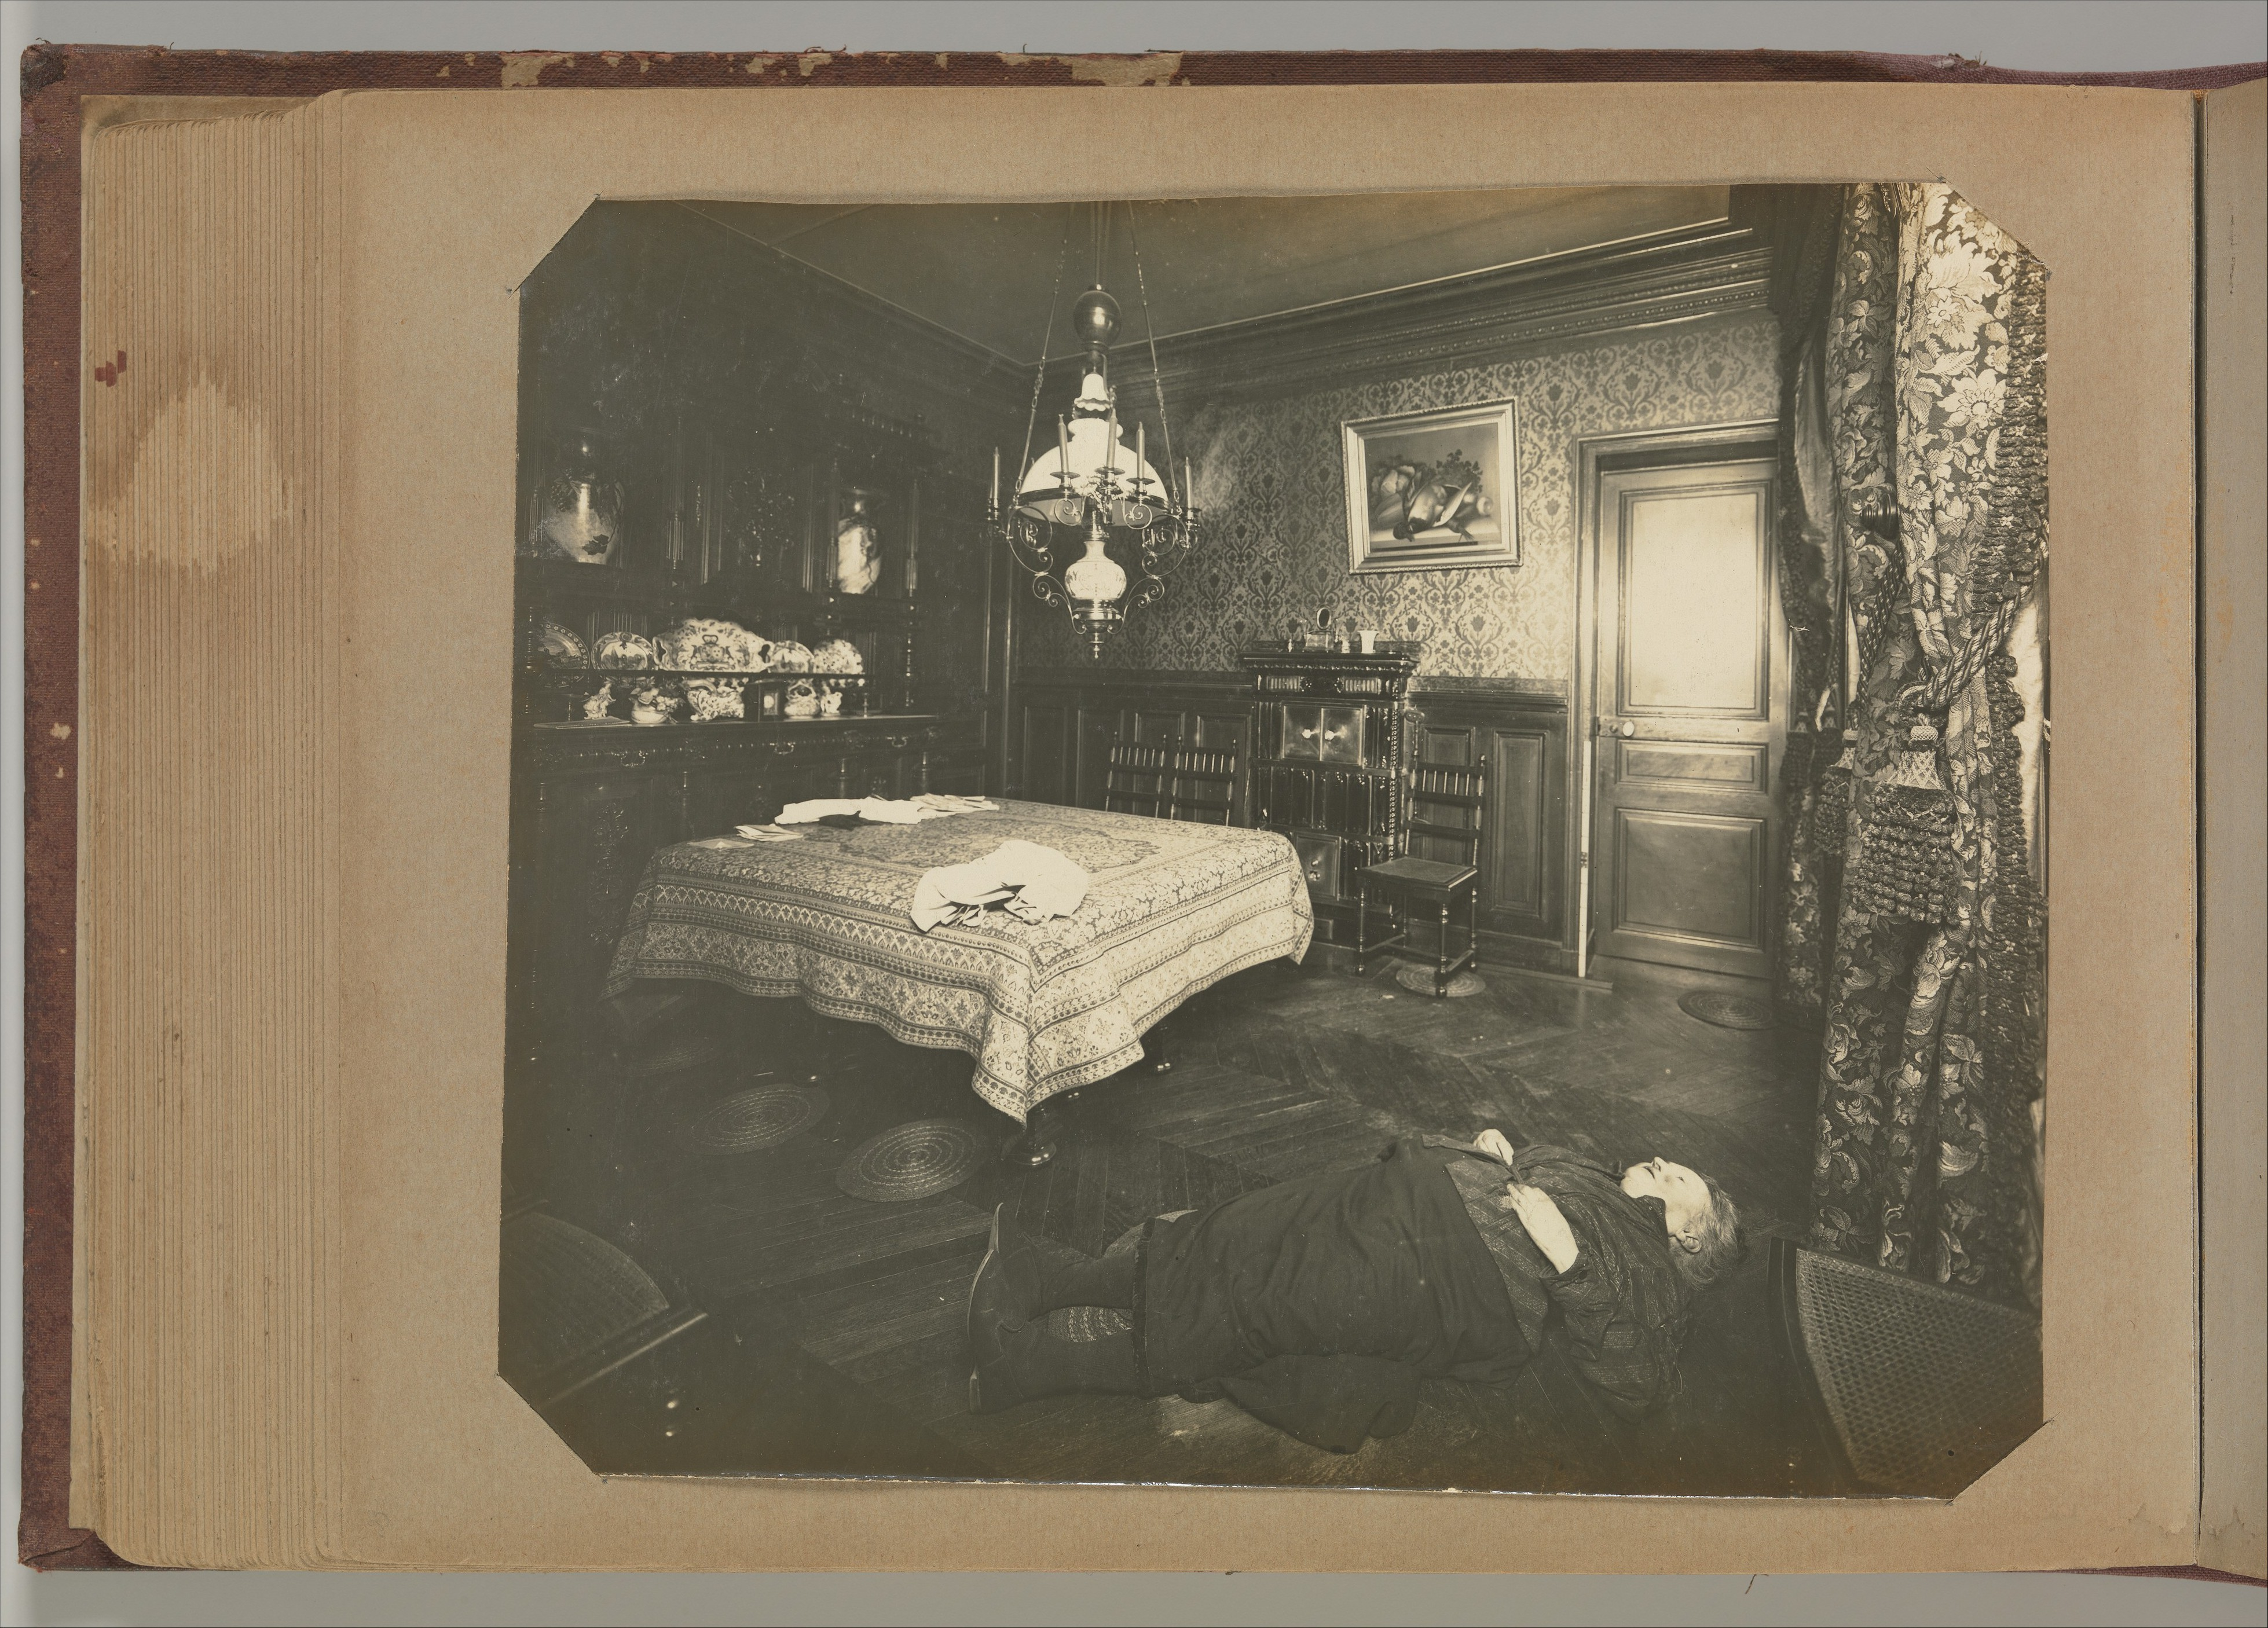
\includegraphics[width=.5\textwidth]{victim.jpg}}
\end{frame}

\begin{frame}{Truth, correspondence, and coherence}
	\begin{itemize}
		\item Coherence Theory 
		\begin{itemize}
			\item Truth is determined by the coherence between new claims and other justified claims
			\item The Defence claims the victim committed suicide.
			\item No history of depression or other mental illness.
			\item Appeared happy
			\item The claim is unlikely to be true, not on the basis of anyone having observed how the injuries were inflicted, but on the lack of coherence between this claim and other justified claims.
		\end{itemize}
	\end{itemize}
	\centerline{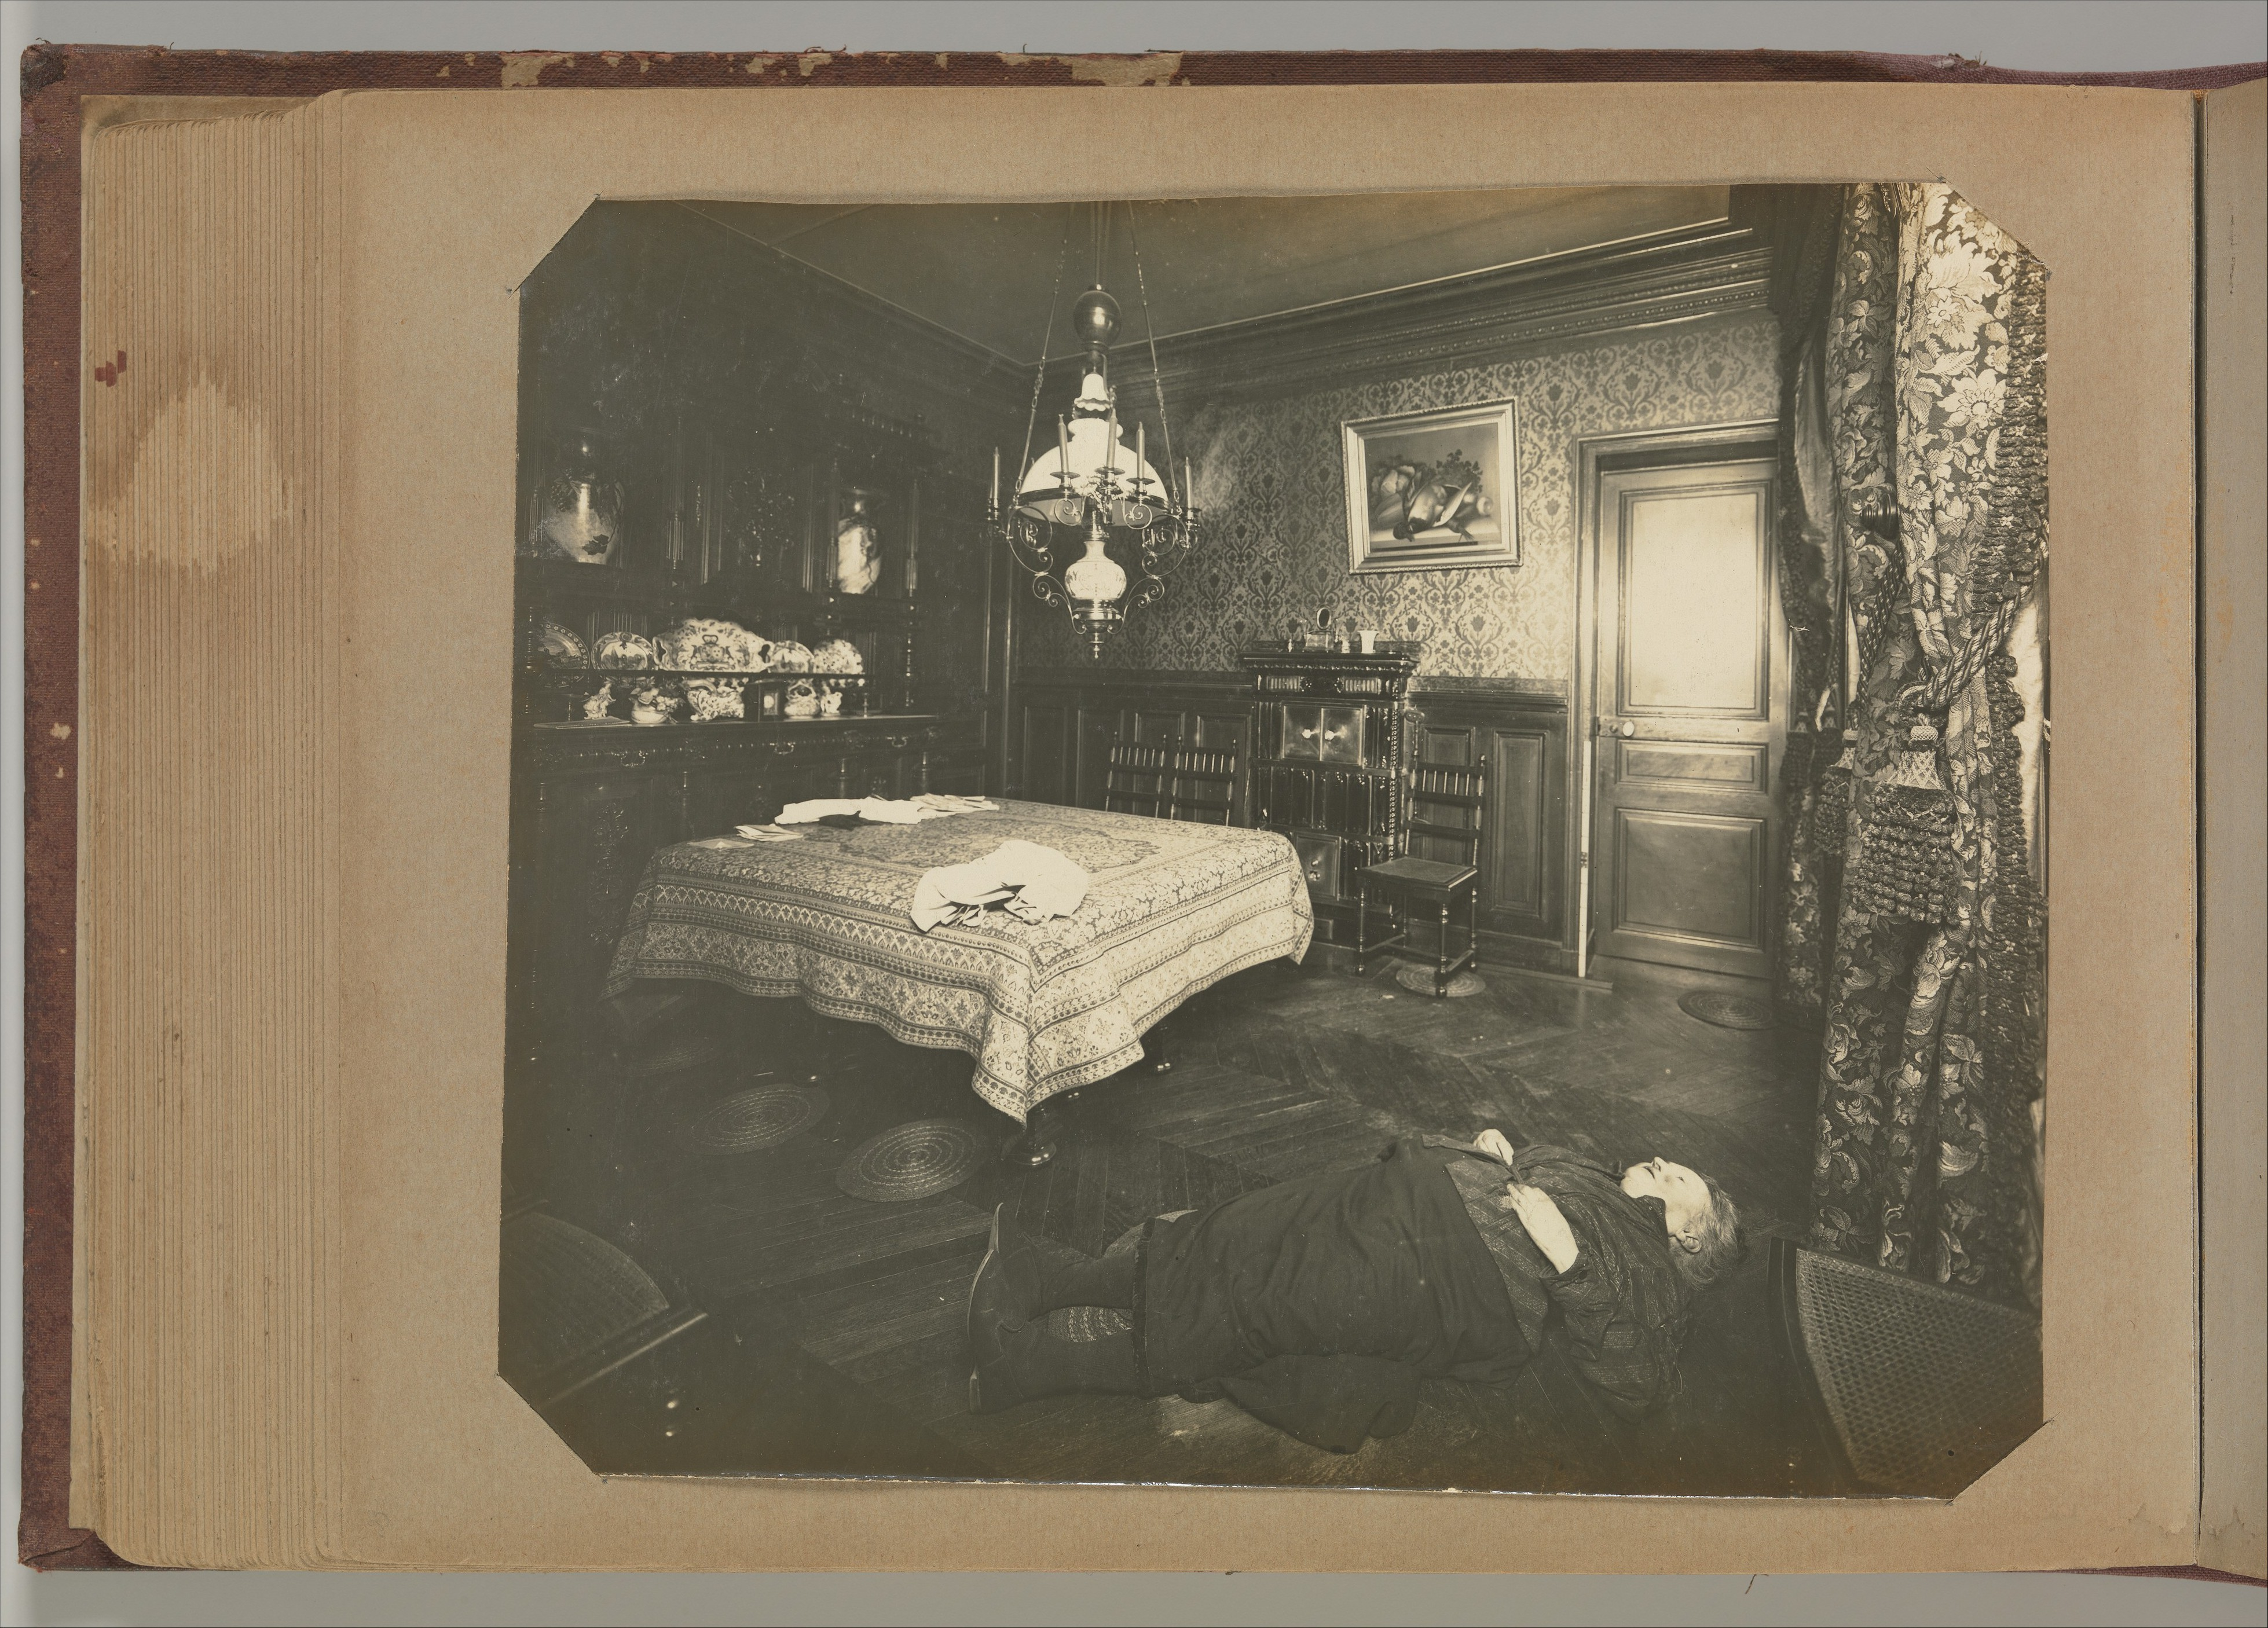
\includegraphics[width=.5\textwidth]{victim.jpg}}
\end{frame}

\begin{frame}{Scientific claims}
	\begin{itemize}
		\item Science is the process of making scientific claims...
		\item ...and determining whether those claims are true or false.
		\item Scientific claims are \textbf{objective} rather than \textbf{subjective}.
		\item Scientific claims are those whose truth can, at least in principle, be clearly determined.
		\item Scientific claims are largely \textbf{descriptive} rather than \textbf{prescriptive}.
	\end{itemize}
\end{frame}

\begin{frame}{Descriptive versus prescriptive claims}
	\begin{itemize}
		\item \textbf{Descriptive claims} say something about how the world is, was, or will be:
		\begin{itemize}
			\item ``Plymouth University was once a polytechnic''
			\item ``Reaction times slow as people age''
			\item ``The UK's Gross Domestic Product will grow by 3\% next year''
		\end{itemize}
	\end{itemize}
\end{frame}


\begin{frame}{Descriptive versus prescriptive claims}
	\begin{itemize}
		\item \textbf{Prescriptive claims} say something about how how things \emph{should} be:
		\begin{itemize}
			\item ``Abortion should be made illegal''
			\item ``People should not drink and drive''
		\end{itemize}
		\item How to examine prescriptive claims scientifically:
		\begin{itemize}
			\item Look for a descriptive claim that might support the prescriptive claim:
			\item \emph{Anti-abortion}: ``feotal pain receptors have developed by eight weeks gestation''
			\item \emph{Pro-abortion}: ``foetal pain receptors are not connected to the brain until 20 weeks''
			\item \emph{Anti-drink-driving}:  ``Risk of car accidents doubles at 80mg/100ml blood alcohol (UK drink-driving limit)''
		\end{itemize}
	\end{itemize}
\end{frame}
			

\begin{frame}{Descriptive versus prescriptive claims}
	\begin{itemize}		
		\item Science is not about avoiding societally difficult questions; nor is it exclusively about societal impact.
		\item It's about making claims that can be reliably examined.
		\begin{itemize}
			\item Some of those claims have direct societal impact (drink driving claims)
			\item Other claims change the way we view ourselves and the world in the longer term.
		\end{itemize}
		\item Quality of science is orthogonal to its ``impact''.
	\end{itemize}
\end{frame}

\begin{frame}{Absolute versus contextual claims}
	\begin{itemize}	
		\item 	\textbf{Absolute claims} are invariant. They hold always. Their truth value is not conditional on circumstances. They are not conditional on time or place.
		\item \textbf{``Relative'' (contextual) claims} hold under a defined set of conditions.
		\begin{itemize}
			\item ``The leadership positions that women occupy are less promising than those of their male counterparts''
			\item Not intended to be an absolute claim.
			\item If the claim is true now, but no longer true in 20 years, this does not undermine the truth value of the original claim.
		\end{itemize}
		\item Scientists generally wish to make claims that are as context-independent as possible; otherwise it is hard to make further predictions.
		\begin{itemize}
			\item ``The leadership positions that women in 2003 in UK FTSE100 companies occupy are less promising than those of their male counterparts''
		\end{itemize}
	\end{itemize}
\end{frame}



\begin{frame}{Scientific claims and truth}
	\begin{itemize}
		\item Some scientific claims are true, others are false.
		\item A claim that is false can still be scientific
	\end{itemize}
\end{frame}

\begin{frame}{Observable, measurable states}
	\begin{itemize}
		\item Scientific claims are based on observable, measurable states
		\item Objective, descriptive claims are not always measurable.
		\item ``Impulsive people are more likely to be criminals''
		\begin{itemize}
			\item Being a criminal is a state that is observable and measurable.
			\item Impulsivity is a vague concept that must be translated into something measurable.
			\item e.g. Barratt Impulsivity Scale.
		\end{itemize}
		\item ``People with one or more criminal convictions score higher on the BIS than people without a conviction''
	\end{itemize}
\end{frame}

\begin{frame}{Independent replication}
	\begin{itemize}
		\item Scientific claims must be expressed in such a way that they permit independent replication.
		\begin{itemize}
			\item ``Willsian Therapy reduces depression''
			\item Wills is the only person who can perform Willsian therapy
			\item The claim is not scientific because any attempt to assess its truth value would have to involve Wills and hence could not be independently replicated.
		\end{itemize}
	\end{itemize}
\end{frame}



\begin{frame}{Scientific claims}
	\begin{enumerate}
		\item \textbf{O}bjective
		\item \textbf{D}escriptive 
		\item \textbf{A}ppropriately context-independent
		\item \textbf{T}rue or false	
		\item \textbf{B}ased on observable measurable states
		\item \textbf{I}ndependent replication
		\item \textbf{F}alsifiable
	\end{enumerate}
\end{frame}

\begin{frame}{Science and dishonesty}
	\begin{itemize}
		\item Dishonesty
		\begin{itemize}
			\item Partially reporting your results (if your intention is obfuscation). 
			\item Choosing a form of data analysis because it gives you the best p-value.
			\item Keeping on testing until p $<$ .05
			\item Publishing the same data more than once.
			\item Making up data!
		\end{itemize}
		\item Dishonesty gets in the way of reliably evaluating claims.
	\end{itemize}
\end{frame}

\begin{frame}{Diderik Stapel}
	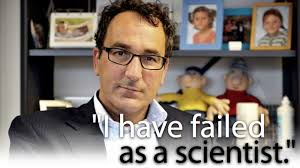
\includegraphics[width=.9\textwidth]{stapel.jpg}

	Dutch social psychologist - admitted to inventing data
	
	See also - Dirk Smeesters - Dutch social psychologist - ``cherry picked'' data.
	
\end{frame}

\begin{frame}{Listening to music about old age reduces your age}
	
	``We asked 20 University of Pennsylvania undergraduates to listen to either 'When I’m Sixty-Four' by The Beatles or 'Kalimba'. Then, in an ostensibly unrelated task, they indicated their birth date (mm/dd/yyyy) and their father’s age. We used father’s age to control for variation in baseline age across participants. An ANCOVA revealed the predicted effect: According to their birth dates, people were nearly a year-and-a-half younger after listening to 'When I’m Sixty-Four' (adjusted M = 20.1 years) rather than to 'Kalimba' (adjusted M = 21.5 years), F(1, 17) = 4.92, p = .040''
	
	\vspace{12 pt}
	
	Simmons et al. (2011, Psychological Science)
	
\end{frame}

\begin{frame}{Science and skepticism}
	\begin{itemize}
		\item Scientists should welcome skepticism.
		\item Scientists should solicit and welcome criticism.
		\item Emotionally quite difficult.
		\item Independent replication
		\begin{itemize}
			\item Scientific claims permit independent replication.
			\item Independent replication should be sought.
			\item High profile failures to replicate...
		\end{itemize}
	\end{itemize}
\end{frame}

\begin{frame}{Ap Dijksterhuis}
	\centerline{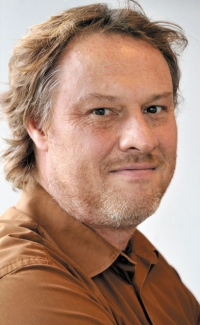
\includegraphics[width=.3\textwidth]{ap.jpg}}

	Dutch social psychologist - his ``intelligence priming'' effects fail to replicate. 
	
	\url{http://www.nature.com/news/disputed-results-a-fresh-blow-for-social-psychology-1.12902}
	
	See also - John Bargh - US social psychologist - his ``age and walking pace'' results fail to replicate
	
\end{frame}


\begin{frame}{Reproducibility project}
	\centerline{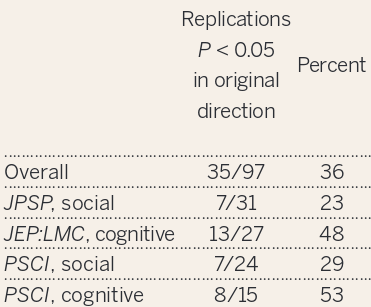
\includegraphics[width=.8\textwidth]{nosek.png}}
	\url{http://www.sciencemag.org/content/349/6251/aac4716}
\end{frame}

\begin{frame}{Science and publication}
	\begin{itemize}
		\item Science is highly social and cooperative.
		\item Collecting data, and evaluating claims, and then keeping the results of that evaluation to yourself is generally frowned upon.
		\item Some scientists would even go so far as to say it is unethical to not publish your work. 
	\end{itemize}
\end{frame}

\begin{frame}{Science and Open Access publication}
	\begin{itemize}
		\item Scientific journals cost \pounds 1000s each per year.
		\item Only held by university libraries, which are not fully open to the public.
		\item Solution: \textbf{Open Access} publishing - making publications freely available at no charge
	\end{itemize}
	\centerline{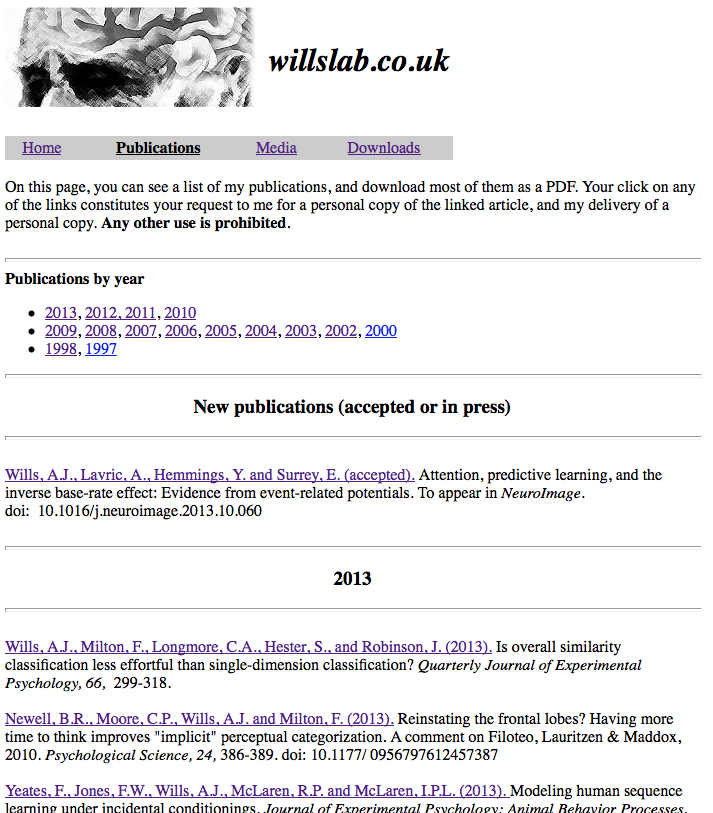
\includegraphics[width=.6\textwidth]{willslab.png}}
\end{frame}

\begin{frame}{Science and Open Access raw data}
	\begin{itemize}
		\item Making your raw data freely, publicly, permanently, available.
		\item Incredibly important. Slowly becoming accepted.
	\end{itemize}
	\centerline{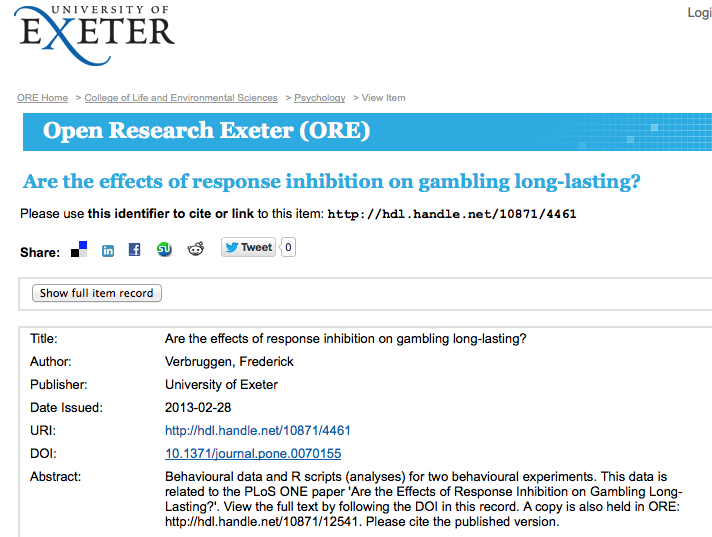
\includegraphics[width=.6\textwidth]{verbruggen.png}}
\end{frame}

\begin{frame}{Science and peer review}
	\begin{itemize}
		\item Evaluation of your work by experts in your sub-field.
		\item Functions of peer review:
		\begin{itemize}
			\item Basic quality control.
			\item Prompts improvements in data and/or analysis.
			\item Prompts improvements in clarity and logic.
			\item Gives an indication of quality (possibly...)
		\end{itemize}
	\end{itemize}
\end{frame}


\begin{frame}{Peer-review process}
	\begin{itemize}
		\item Process
		\begin{enumerate}
			\item Submit paper
			\item Receive 2-3 reviews
			\item Editorial decision: Accept / revise and resubmit / reject
			\item Submit revised paper
			\item Likely receive further reviews
			\item Editorial final decision
		\end{enumerate}
		\item Duration
		\begin{itemize}
			\item Rejection: 24 hours --- 9 months.
			\item Acceptance: 3 months --- 2 years. 
			\item Often, you send to more than one journal (see indication of quality)
		\end{itemize}
		\item Controversy
		\begin{itemize}
			\item Peer review is traditionally closed and anonymous
			\item Is open and named a better model?
		\end{itemize}
	\end{itemize}
\end{frame}

\begin{frame}{Behavioral and Brain Sciences}
	\centerline{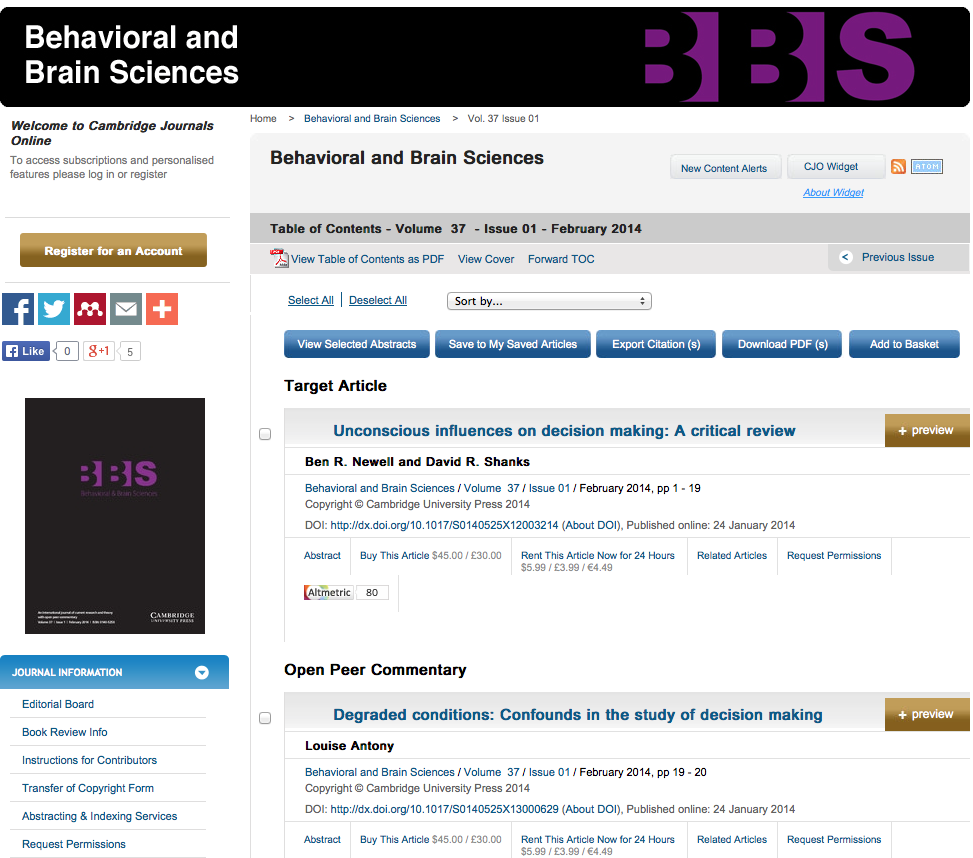
\includegraphics[width=.8\textwidth]{bbs.png}}
\end{frame}	

\begin{frame}{Culture of modern science (and future directions)}
	\begin{itemize}
		\item Evaluation of scientific claims
		\item Honesty
		\item Skepticism	(Independent replication?)
		\item Publication	 (Open Access? Raw data?)
		\item Peer review	 (Named? Open?) 
	\end{itemize}
	\vspace{12pt}

\tiny
This work is licensed under a Creative Commons Attribution-ShareAlike
4.0 International Licence. Last update: \today
	
\end{frame}

\end{document}



%%% Local Variables:
%%% mode: latex
%%% TeX-master: t
%%% End:
